\documentclass[final]{ua-thesis}
% \documentclass[School=Harvard]{Harvard_Princeton_NYU}
% \documentclass{SPhdThesis}
% \documentclass[draft]{ua-thesis}
% \documentclass[conference,compsoc]{IEEEtran}
% \documentclass[3p,,preprint,12pt]{elsarticle}

% \usepackage{verbatim, amssymb, amsmath, amsthm, graphicx, psfrag, afterpage, subfigure, hyperref}
\usepackage[mathscr]{eucal}
\usepackage{makeidx}
\numberwithin{equation}{section}
%====================================================================
%-------------------------------------------------------------------- 
%
%   isomath.tex  LaTeX macros for math conforming to ISO standards
%
%---------------------------------------- this is a LaTeX-2e document
%====================================================================     

%% Blackboard Bold

\newcommand*{\bbb}[1]{\mathbb{#1}}
\newcommand{\bC}{\bbb{C}}
\newcommand{\bN}{\bbb{N}}
\newcommand{\bQ}{\bbb{Q}}
\newcommand{\bR}{\bbb{R}}
\newcommand{\bZ}{\bbb{Z}}
\newcommand{\bF}{\bbb{F}}
\newcommand{\bFp}{\bbb{F}_p}
\newcommand{\bFpn}{\bbb{F}_{p^n}}
\newcommand{\ii}{\mathbf{i}}
\newcommand{\jj}{\mathbf{j}}
\newcommand{\kk}{\mathbf{k}}

\newcommand{\N}{\bN}
\newcommand{\Q}{\bQ}
\newcommand{\R}{\bR}
\newcommand{\Z}{\bZ}
\newcommand{\ZpZ}{\Z/p\Z}
\newcommand{\ZmZ}{\Z/m\Z}
\newcommand{\C}{\bC}
%\newcommand{\F}{\bF}
\newcommand{\F}{\mathbb{F}}
\newcommand{\Fp}{\bFp}
\newcommand{\Fpn}{\bFpn}

%% Calligraphic

\newcommand{\mC}{\mathcal{C}}
\newcommand{\mT}{\mathcal{T}}

%% Miscellaneous

%% Named Functions and Operators

\newcommand{\id}{\mathrm{id}}
\newcommand{\Id}{\mathrm{Id}}
\newcommand{\rank}{\mathrm{rank}}
\newcommand{\supp}{\mathrm{supp}}
\newcommand{\tr}{\mathrm{tr}}
\newcommand{\Aut}{\mathrm{Aut}}
\newcommand{\Gal}{\mathrm{Gal}}
\newcommand{\Hom}{\mathrm{Hom}}
\newcommand{\im}{\mathrm{im}}
\newcommand{\lcm}{\mathrm{lcm}}
\newcommand{\Tr}{\mathrm{Tr}}
\newcommand{\GL}{\mathrm{GL}}
%\newcommand{\mod}{\textrm{ mod }}

%% Vectors

\usepackage{amsbsy}
\renewcommand*{\vec}[1]{\boldsymbol{#1}}
\newcommand{\va}{\vec{a}}
\newcommand{\vb}{\vec{b}}
\newcommand{\vc}{\vec{c}}
\newcommand{\vx}{\vec{x}}
\newcommand{\vy}{\vec{y}}
\newcommand{\vz}{\vec{z}}
\newcommand{\vu}{\vec{u}}
% \newcommand{\vv}{\vec{v}}
\newcommand{\vw}{\vec{w}}

%% Logical Propositions

\newcommand*{\pro}[1]{\mathsf{#1}}
\newcommand{\pP}{\pro{P}}
\newcommand{\pQ}{\pro{Q}}
\newcommand{\pR}{\pro{R}}

%% Matrices and Tensors

%\DeclareMathAlphabet{\mathsfsl}{OT1}{cmss}{m}{sl}
\newcommand*{\mat}[1]{\mathsfsl{#1}}
\newcommand{\mM}{\mat{M}}
\newcommand{\mD}{\mat{D}}
\newcommand{\mI}{\mat{I}}

%% Special Numbers and Characters

\newcommand{\re}{\mathrm{e}}
\newcommand{\ri}{\mathrm{i}}
\newcommand{\rd}{\mathrm{d}} % differential
\newcommand{\dif}[1]{\,\rd{#1}} % differential
\newcommand{\df}{\dif{f}}
\newcommand{\dx}{\dif{x}}
\newcommand{\dy}{\dif{y}}
\newcommand{\dz}{\dif{z}}
\newcommand{\dt}{\dif{t}}
\newcommand{\rpi}{\pi}       % actually, pi should be upright.

\newcommand{\rE}{\mathsf{E}}
\newcommand{\rF}{\mathsf{F}}
\newcommand{\rI}{\mathsf{I}}
\newcommand{\rK}{\mathsf{K}}
\newcommand{\rL}{\mathsf{L}}
\newcommand{\rM}{\mathsf{M}}
\newcommand{\rN}{\mathsf{N}}
\newcommand{\rP}{\mathsf{P}}
\newcommand{\rT}{\mathsf{T}}
\newcommand{\rU}{\mathsf{U}}
\newcommand{\rV}{\mathsf{V}}
\newcommand{\rW}{\mathsf{W}}
\newcommand{\rX}{\mathsf{X}}
\newcommand{\rY}{\mathsf{Y}}
\newcommand{\rZ}{\mathsf{Z}}

%====================================================================
%
%  mathenv.tex  math environments  version 0.00
%
%====================================================================

\usepackage{ifthen}

\theoremstyle{plain}
%\newtheorem{thm}{Theorem}[subsection]
\newtheorem{thm}[equation]{Theorem}
\newtheorem{cor}[equation]{Corollary}
\newtheorem{lem}[equation]{Lemma}
\newtheorem{prop}[equation]{Proposition}
\newtheorem{ax}[equation]{Axiom}
\newtheorem*{thm*}{Theorem}
\newtheorem*{cor*}{Corollary}
\newtheorem*{lem*}{Lemma}
\newtheorem*{prop*}{Proposition}
\newtheorem*{ax*}{Axiom}

\theoremstyle{definition}
\newtheorem{defn}[equation]{Definition}
\newtheorem{problem}{Problem}
\newtheorem*{defn*}{Definition}
\newtheorem*{problem*}{Problem}
\newtheorem{ex}[equation]{Example}
\newtheorem{exs}[equation]{Examples}
\newtheorem*{ex*}{Example}
\newtheorem*{exs*}{Examples}

%\theoremstyle{remark}
\newtheorem{rem}[equation]{Remark}
\newtheorem*{rem*}{Remark}
\newtheorem{aside}[equation]{Aside}
\newtheorem*{aside*}{Aside}
\newtheorem{intuition}[equation]{Intuition}
\newtheorem*{intuition*}{Intuition}
\newtheorem{notn}[equation]{Notation}
\newtheorem*{notn*}{Notation}
\newtheorem{conv}[equation]{Convention}
\newtheorem*{conv*}{Convention}
\newtheorem{interp}[equation]{Interpretation}
\newtheorem*{interp*}{Interpretation}
\newtheorem{mnem}[equation]{Mnemonic}
\newtheorem*{mnem*}{Mnemonic}
\newtheorem{exer}[equation]{Exercise}
\newtheorem*{exer*}{Exercise}
\newtheorem{conjecture}[equation]{Conjecture}
\newtheorem*{conjecture*}{Conjecture}

%\numberwithin{equation}{subsection}
%\numberwithin{equation}{section}

%\newcommand{\beginex}{\begin{ex}$\blacktriangleright$ }
%\newcommand{\mendex}{\hfill$\blacktriangleleft$\end{ex}}
\newcommand{\beginex}{\begin{ex}$\rhd$ }
\newcommand{\mendex}{\hfill$\lhd$\end{ex}}

%--------------------------------------------------------------------
%
%\newenvironment{problem}[1][]
% {\noindent{\bf#1.\ }}
% {}
%
%--------------------------------------------------------------------

\newenvironment{answer}[1][Answer]
  {\begin{proof}[#1]}
  {\renewcommand{\qedsymbol}{}\end{proof}}

\newenvironment{solution}[1][Solution]
  {\begin{proof}[#1]}
  {\renewcommand{\qedsymbol}{\ensuremath{\Diamond}}\end{proof}}

\newcounter{ppart}
\newenvironment{parts}
 {\begin{list}{\textup(\alph{ppart}\textup)\hfill}
   {\usecounter{ppart}
    \settowidth{\labelwidth}{\textup(m\textup)}
    \setlength{\leftmargin}{0cm} 
    \setlength{\rightmargin}{0cm}
    \setlength{\itemindent}{2em}
    \setlength{\labelsep}{\itemindent}
    \addtolength{\labelsep}{-\labelwidth}
    \renewcommand{\makelabel}[1]{\ifthenelse
     {\equal{##1}{}}
     {\textup{(\alph{ppart})}\hfill}
     {\textup{##1}\hfill}}
   }
 }
 {\end{list}}

%\renewcommand{\labelenumi}{(\roman{enumi})}

\newcommand{\secref}[1]{Section~\textup{\ref{#1}}}
\newcommand{\thmref}[1]{Theorem~\textup{\ref{#1}}}
\newcommand{\corref}[1]{Corollary~\textup{\ref{#1}}}
\newcommand{\lemref}[1]{Lemma~\textup{\ref{#1}}}
\newcommand{\propref}[1]{Proposition~\textup{\ref{#1}}}
\newcommand{\defnref}[1]{Definition~\textup{\ref{#1}}}
\newcommand{\remref}[1]{Remark~\textup{\ref{#1}}}
\newcommand{\exref}[1]{Example~\textup{\ref{#1}}}
\newcommand{\exsref}[1]{Examples~\textup{\ref{#1}}}
\newcommand{\axref}[1]{Axiom~\textup{\ref{#1}}}
\newcommand{\itemref}[1]{\textup{{\ref{#1}}}}

% Vim 7.0 syntax highlighting doesn't seem to kick in unless the .tex
% file has at least one begin-end pair in it.  Go figure.
\newenvironment{vim_bug_workaround}
	{}

%====================================================================


\newcommand*{\ds}[1]{\displaystyle{#1}}

\newcommand*{\bfidx}[1]{\index{#1}\textbf{#1}}
\newcommand*{\bfidxtwo}[2]{\textbf{#1}\index{#2}}
\newcommand*{\bfidxaux}[2]{\index{#1}\index{#2}\textbf{#1}}
\newcommand*{\emphidx}[1]{\index{#1}\emph{#1}}
\newcommand*{\plainidx}[1]{\index{#1}#1}

\newcommand*{\bra}[1]{\langle \, #1 \mid}
\newcommand*{\ket}[1]{\mid #1 \, \rangle}
\newcommand*{\braket}[2]{\langle #1 \mid #2 \rangle}
\newcommand*{\braCket}[3]{\langle #1 \mid #2 \mid #3 \rangle}
\newcommand*{\BraCKet}[3]
	{\Bigg\langle #1 \,\Bigg|\, #2 \,\Bigg|\, #3 \Bigg\rangle}
\newcommand*{\expn}[1]{\langle \, #1 \, \rangle}
\newcommand*{\ketbra}[1]{\ket{ #1 } \bra{ #1 }}
\newcommand*{\TrebH}{\Tr\left(e^{-\beta H}\right)}
\newcommand*{\TrXebH}[1]{\Tr\left(#1 e^{-\beta H}\right)}
\newcommand*{\Trsym}{\Tr_{L^2_{\mathrm{sym}}}}
\newcommand*{\intRdntimes}[2]{\underbrace{
	\int_{\R^{#1}} \int_{\R^{#1}} \cdots \int_{\R^{#1}}}_{#2 \textrm{ times}}}

\newcommand{\lmax}{\ell_{\textrm{max}}}

\newcommand{\ellx}{\ell_{\vecx}}
\newcommand{\elly}{\ell_{\vecy}}

\newcommand{\ellxpi}{\ell_{\vecx}(\pi)}
\newcommand{\ellypi}{\ell_{\vecy}(\pi)}

\newcommand{\ellxpiprime}{\ell_{\vecx}(\pi')}
\newcommand{\ellypiprime}{\ell_{\vecy}(\pi')}

\newcommand{\ellxypi}{\ell_{\vecx,\vecy}(\pi)}
\newcommand{\ellyxpi}{\ell_{\vecy,\vecx}(\pi)}

\newcommand{\essx}{s_{\vecx}}

\newcommand{\essxpi}{s_{\vecx}(\pi)}

\newcommand{\ellxf}{\ell^f_{\vecx}}
\newcommand{\essxf}{s^f_{\vecx}}
\newcommand{\ellmax}{\ell_{\textrm{max}}}
\newcommand{\fM}{f_{\textrm{max}}}
\newcommand{\ellbar}{\overline{\ell}}
\newcommand{\ellfbar}{\overline{\ell}_f}
\newcommand{\essbar}{\overline{s}}
\newcommand{\essfbar}{\overline{s}_f}

\newcommand{\rhocz}{\rho_c^{(0)}}
\newcommand{\rhocal}{\rho_c^{(\alpha)}}
\newcommand{\betacz}{\beta_c^{(0)}}
\newcommand{\betacal}{\beta_c^{(\alpha)}}
\newcommand{\Tcz}{T_c^{(0)}}
\newcommand{\Tcal}{T_c^{(\alpha)}}

\newcommand{\Xt}{X_t}
\newcommand{\Yt}{Y_t}
\newcommand{\Xtk}{X_{t+k}}
\newcommand{\Ytk}{Y_{t+k}}

\newcommand{\cmhat}{\hat{c}_m}
\newcommand{\chat}{\hat{c}}
\newcommand{\tauint}{{\tau_{\textrm{int}}}}
\newcommand{\hattauint}{\hat{\tau}_{\textrm{int}}}
\newcommand{\tauexp}{{\tau_{\textrm{exp}}}}
\newcommand{\stilde}{{\tilde{s}}}
\newcommand{\ttilde}{{\tilde{t}}}

\newcommand{\sumiB}{\sum_{i=0}^{B-1}}
\newcommand{\sumjB}{\sum_{j=0}^{B-1}}
\newcommand{\sumiM}{\sum_{i=0}^{M-1}}
\newcommand{\sumjM}{\sum_{j=0}^{M-1}}
\newcommand{\sumiN}{\sum_{i=0}^{N-1}}
\newcommand{\sumjN}{\sum_{j=0}^{N-1}}

%% ----------------------------------------------------------------
\def\ve{\varepsilon}
\def\veps{\varepsilon}
\def\bbB{\mathbb{B}}
\def\bbE{\mathbb{E}}
\def\bbP{\mathbb{P}}
\def\muhat{\hat{\mu}}
\def\psihat{\hat{\psi}}
\def\fhat{\hat{f}}
\def\ghat{\hat{g}}
\def\Ahat{\hat{A}}
\def\Fhat{\hat{F}}
\def\Hhat{\hat{H}}
\def\What{\hat{W}}
\def\Yhat{\hat{Y}}
\def\Zhat{\hat{Z}}
\def\nuhat{\hat{\nu}}
\def\rhohat{\hat{\rho}}
\def\Xihat{\hat{Xi}}
\def\xbar{\overline{x}}
%\def\torusdiff{\tilde{\vecd}}
\def\torusdiff{\vecd_\Lambda}

\def\muX{\mu_{X}}
\def\muY{\mu_{Y}}
\def\muXNbar{\mu_{\overline{X}_N}}
\def\muYNbar{\mu_{\overline{Y}_N}}
\def\sigmaX{\sigma_{X}}
\def\sigmaY{\sigma_{Y}}
\def\sigmaXNbar{\sigma_{\overline{X}_N}}
\def\sigmaYNbar{\sigma_{\overline{Y}_N}}

\def\ANbar{{\overline{A}_N}}

\def\QMbar{{\overline{Q}_M}}

\def\Xbar{\overline{X}}
\def\XNbar{{\overline{X}_N}}
\def\XMbar{{\overline{X}_M}}
\def\XNBbar{{\overline{X}_{N,B}}}

\def\Ybar{\overline{Y}}
\def\YNbar{\overline{Y}_N}
\def\YNBbar{\overline{Y}_{N,B}}

\def\Z{\mathbb{Z}}

\def\Htilde{\tilde{H}}
\def\Halpha{H^{(\alpha)}}
\def\HP{H_P}
\def\HPzero{H_P^{(0)}}
\def\HPone{H_P^{(1)}}

\def\bfH{\mathbf{H}}
\def\bfx{\mathbf{x}}

\def\bsH{\mathbf{H}}
\def\bsx{\mathbf{x}}

\def\caS{\mathcal{S}}
\def\mcS{\mathcal{S}}

\def\mcF{\mathcal{F}}
\def\mcK{\mathcal{K}}
\def\mcL{\mathcal{L}}
\def\mcH{\mathcal{H}}
\def\mcN{\mathcal{N}}
\def\mcO{\mathcal{O}}

\def\msH{\mathscr{H}}
\newcommand*{\pig}[1]{\langle #1 \rangle}
\newcommand*{\pigm}[1]{\langle #1 \rangle_M}

%% ----------------------------------------------------------------
\newcommand{\Sn}{\mathcal{S}_n}
\newcommand{\SN}{\mathcal{S}_N}
\newcommand{\SNp}{\mathcal{S}_{N+1}}
\newcommand{\SNpc}{{\SNp \setminus \SN}}
\newcommand{\dd}{\mathrm{d}}
\newcommand{\e}{\mathrm{e}}
\newcommand{\Var}{\mathrm{Var}}
\newcommand{\Corr}{\mathrm{Corr}}
\newcommand{\Cov}{\mathrm{Cov}}

%% ----------------------------------------------------------------
\def\veca{\mathbf{a}}
\def\vecb{\mathbf{b}}
\def\vecc{\mathbf{c}}
\def\vecd{\mathbf{d}}
\def\vecg{\mathbf{g}}
\def\veck{\mathbf{k}}
\def\vecm{\mathbf{m}}
\def\vecn{\mathbf{n}}
\def\vecr{\mathbf{r}}
\def\vecu{\mathbf{u}}
\def\vecv{\mathbf{v}}
\def\vecw{\mathbf{w}}
\def\vecx{\mathbf{x}}
\def\vecy{\mathbf{y}}
\def\vecz{\mathbf{z}}

\def\vecK{\mathbf{K}}
\def\vecM{\mathbf{M}}
\def\vecP{\mathbf{P}}
%\def\vecP{\mathcal{P}}
\def\vecV{\mathbf{V}}
\def\vecW{\mathbf{W}}
\def\vecWhat{\hat{\mathbf{W}}}
\def\vecX{\mathbf{X}}
\def\vecY{\mathbf{Y}}
\def\vecZ{\mathbf{Z}}

\def\vecPpiz{\vecP^{(\pi_0)}}
\def\Ppiz{P^{(\pi_0)}}
\def\P{P_{\mathrm{Gibbs}}}
\def\Phat{\hat{P}_{\mathrm{Gibbs}}}

%\def\mkvM{\mathbf{M}}
%\def\mkvM{R}
\def\mkvM{A}
%\def\mkvM{\mathcal{M}}

\newcommand{\vecomega}{{\boldsymbol{\omega}}}
\newcommand{\vecmu}{{\boldsymbol{\mu}}}
\newcommand{\vecnu}{{\boldsymbol{\nu}}}

\def\vecxi{\mathbf{x}_{i}}
\def\vecxj{\mathbf{x}_{j}}
\def\vecxpii{\mathbf{x}_{\pi(i)}}
\def\vecxpij{\mathbf{x}_{\pi(j)}}
\def\vecxpik{\mathbf{x}_{\pi(k)}}
\def\veckpii{\mathbf{k}_{\pi(i)}}

\def\pii{\pi^{-1}}
\def\piinv{\pi^{-1}}

\def\pix{\pi(\vecx)}
\def\piy{\pi(\vecy)}

\def\piprimex{\pi'(\vecx)}
\def\piprimey{\pi'(\vecy)}

\def\piv{\pi(\vecv)}
\def\piw{\pi(w)}
\def\piiw{\pi^{-1}(w)}
\def\piix{\pi^{-1}(\vecx)}
\def\piiy{\pi^{-1}(\vecy)}
\def\edh{e^{-\Delta H}}

\def\vecwi{\mathbf{w}^{(i)}}
\def\vecwj{\mathbf{w}^{(j)}}
\def\vecwk{\mathbf{w}^{(k)}}
\def\vecwij{\mathbf{w}^{(ij)}}

\def\vecwil{\mathbf{w}^{(i_\ell)}}
\def\vecwjl{\mathbf{w}^{(j_\ell)}}

\def\xhat{\hat{x}}
\def\yhat{\hat{y}}

\DeclareMathOperator*{\ctdto}{\circ\hspace{-0.2mm}--\hspace{-0.3mm}\circ}
\DeclareMathOperator*{\notctdto}{\circ\hspace{-0.2mm}--\hspace{-2.5mm}\not--\hspace{-0.3mm}\circ}
\def\maybeeq{\stackrel{?}{=}}
\DeclareMathOperator*{\twocyc}{\circ\hspace{-0.2mm}-\pi-\hspace{-0.4mm}\circ}
\DeclareMathOperator*{\ntwocyc}{\circ\hspace{-0.2mm}-\not\pi-\hspace{-0.4mm}\circ}


%% ----------------------------------------------------------------
\newcommand{\tand}{\textrm{and}}
\newcommand{\qand}{\quad\textrm{and}\quad}
\newcommand{\qqand}{\qquad\textrm{and}\qquad}
\newcommand{\qor}{\quad\textrm{or}\quad}
\newcommand{\qqor}{\qquad\textrm{or}\qquad}
\newcommand{\qie}{\quad\textrm{i.e.}\quad}
\newcommand{\qqie}{\qquad\textrm{i.e.}\qquad}
\newcommand{\qqwith}{\qquad\textrm{with}\qquad}

%% ================================================================
%\newcommand{\Suto}{S\"ut\H{o}}
\def\Suto{S\"ut\H{o}}

\newcommand{\grad}{\nabla}
\newcommand{\tensor}{\otimes}
\newcommand{\into}{\hookrightarrow}
\newcommand{\longto}{\longrightarrow}
\def\upto{\nearrow}
\newcommand{\ix}{\pi(x)}
\newcommand{\iy}{\pi^{-1}(y)}
\newcommand{\iu}{\pi(u)}
\newcommand{\tat}{\textasciitilde}

\newcommand*{\boxalign}[1]{
	\begin{equation*}
	\addtolength{\fboxsep}{5pt}
	\boxed{
	\begin{aligned}
	#1
	\end{aligned}
	}
	\end{equation*}
}

\newcommand*{\rowvectwo}[2]{\begin{pmatrix}#1 & #2 \end{pmatrix}}
\newcommand*{\rowvecthree}[3]{\begin{pmatrix}#1 & #2 & #3\end{pmatrix}}

\newcommand*{\colvecone}[1]{\left(\begin{array}{r} #1 \end{array}\right)}
\newcommand*{\colvectwo}[2]{\left(\begin{array}{r} #1 \\ #2 \end{array}\right)}
\newcommand*{\colvecthree}[3]{\left(\begin{array}{r} #1 \\ #2 \\ #3\end{array}\right)}
\newcommand*{\colvecfour}[4]{\left(\begin{array}{r} #1 \\ #2 \\ #3 \\ #4\end{array}\right)}

\newcommand*{\collvecone}[1]{\left(\begin{array}{l} #1 \end{array}\right)}
\newcommand*{\collvectwo}[2]{\left(\begin{array}{l} #1 \\ #2 \end{array}\right)}
\newcommand*{\collvecthree}[3]{\left(\begin{array}{l} #1 \\ #2 \\ #3\end{array}\right)}
\newcommand*{\collvecfour}[4]{\left(\begin{array}{l} #1 \\ #2 \\ #3 \\ #4\end{array}\right)}

\newcommand*{\colcvecone}[1]{\left(\begin{array}{c} #1 \end{array}\right)}
\newcommand*{\colcvectwo}[2]{\left(\begin{array}{c} #1 \\ #2 \end{array}\right)}
\newcommand*{\colcvecthree}[3]{\left(\begin{array}{c} #1 \\ #2 \\ #3\end{array}\right)}
\newcommand*{\colcvecfour}[4]{\left(\begin{array}{c} #1 \\ #2 \\ #3 \\ #4\end{array}\right)}

\newcommand*{\colrvecone}[1]{\left(\begin{array}{r} #1 \end{array}\right)}
\newcommand*{\colrvectwo}[2]{\left(\begin{array}{r} #1 \\ #2 \end{array}\right)}
\newcommand*{\colrvecthree}[3]{\left(\begin{array}{r} #1 \\ #2 \\ #3\end{array}\right)}
\newcommand*{\colrvecfour}[4]{\left(\begin{array}{r} #1 \\ #2 \\ #3 \\ #4\end{array}\right)}

%% ----------------------------------------------------------------
\newcommand{\D}{\partial}
\newcommand{\DA}{\partial A}
\newcommand{\DB}{\partial B}
\newcommand{\DC}{\partial C}
\newcommand{\DX}{\partial X}
\newcommand{\Dc}{\partial c}
\newcommand{\Df}{\partial f}
\newcommand{\Dg}{\partial g}
\newcommand{\DG}{\partial G}
\newcommand{\Dh}{\partial h}
\newcommand{\DM}{\partial M}
\newcommand{\Dr}{\partial r}
\newcommand{\Du}{\partial u}
\newcommand{\Dx}{\partial x}
\newcommand{\Dy}{\partial y}
\newcommand{\Dz}{\partial z}
\newcommand{\Ds}{\partial s}
\newcommand{\Dt}{\partial t}

\newcommand{\DD}{\partial/\partial}
\newcommand{\DDA}{\partial/\partial A}
\newcommand{\DDB}{\partial/\partial B}
\newcommand{\DDC}{\partial/\partial C}
\newcommand{\DDX}{\partial/\partial X}
\newcommand{\DDc}{\partial/\partial c}
\newcommand{\DDf}{\partial/\partial f}
\newcommand{\DDg}{\partial/\partial g}
\newcommand{\DDG}{\partial/\partial G}
\newcommand{\DDh}{\partial/\partial h}
\newcommand{\DDM}{\partial/\partial M}
\newcommand{\DDr}{\partial/\partial r}
\newcommand{\DDx}{\partial/\partial x}
\newcommand{\DDy}{\partial/\partial y}
\newcommand{\DDz}{\partial/\partial z}
\newcommand{\DDs}{\partial/\partial s}
\newcommand{\DDt}{\partial/\partial t}

%% ----------------------------------------------------------------
\newcommand*{\slashD}[1]{\partial/\partial #1}
\newcommand*{\fracD}[1]{\frac{\partial}{\partial #1}}
\newcommand*{\slashDtwo}[2]{\partial #1/\partial #2}
\newcommand*{\fracDtwo}[2]{\frac{\partial #1}{\partial #2}}

\newcommand{\slashDx}{\partial/\partial x}
\newcommand{\slashDy}{\partial/\partial y}
\newcommand{\slashDz}{\partial/\partial z}

\newcommand{\fracDs}{\frac{\partial}{\partial s}}
\newcommand{\fracDt}{\frac{\partial}{\partial t}}
\newcommand{\fracDx}{\frac{\partial}{\partial x}}
\newcommand{\fracDy}{\frac{\partial}{\partial y}}
\newcommand{\fracDz}{\frac{\partial}{\partial z}}
\newcommand{\fracDxx}{\frac{\partial^2}{\partial x^2}}

\newcommand{\fracDfx}{\frac{\partial f}{\partial x}}
\newcommand{\fracDfy}{\frac{\partial f}{\partial y}}
\newcommand{\fracDfz}{\frac{\partial f}{\partial z}}

\newcommand{\fracDgt}{\frac{\partial g}{\partial t}}
\newcommand{\fracDgu}{\frac{\partial g}{\partial u}}
\newcommand{\fracDguu}{\frac{\partial^2 g}{\partial u^2}}
\newcommand{\fracDgv}{\frac{\partial g}{\partial v}}
\newcommand{\fracDgvv}{\frac{\partial^2 g}{\partial v^2}}
\newcommand{\fracDguv}{\frac{\partial^2 g}{\partial u \partial v}}

\newcommand{\fracDht}{\frac{\partial h}{\partial t}}
\newcommand{\fracDhu}{\frac{\partial h}{\partial u}}
\newcommand{\fracDhuu}{\frac{\partial^2 h}{\partial u^2}}
\newcommand{\fracDhv}{\frac{\partial h}{\partial v}}
\newcommand{\fracDhvv}{\frac{\partial^2 h}{\partial v^2}}
\newcommand{\fracDhuv}{\frac{\partial^2 h}{\partial u \partial v}}

\newcommand{\fracDgx}{\frac{\partial g}{\partial x}}
\newcommand{\fracDgxx}{\frac{\partial^2 g}{\partial x^2}}
\newcommand{\fracDgy}{\frac{\partial g}{\partial y}}
\newcommand{\fracDgyy}{\frac{\partial^2 g}{\partial y^2}}
\newcommand{\fracDgz}{\frac{\partial g}{\partial z}}
\newcommand{\fracDgxy}{\frac{\partial^2 g}{\partial x \partial y}}

\newcommand{\fracDhx}{\frac{\partial h}{\partial x}}
\newcommand{\fracDhxx}{\frac{\partial^2 h}{\partial x^2}}
\newcommand{\fracDhy}{\frac{\partial h}{\partial y}}
\newcommand{\fracDhyy}{\frac{\partial^2 h}{\partial y^2}}
\newcommand{\fracDhz}{\frac{\partial h}{\partial z}}
\newcommand{\fracDhxy}{\frac{\partial^2 h}{\partial x \partial y}}

\newcommand{\fracDphis}{\frac{\partial    \phi}{\partial s}}
\newcommand{\fracDphit}{\frac{\partial    \phi}{\partial t}}
\newcommand{\fracDphix}{\frac{\partial    \phi}{\partial x}}
\newcommand{\fracDphixx}{\frac{\partial^2 \phi}{\partial x^2}}
\newcommand{\fracDphiy}{\frac{\partial    \phi}{\partial y}}
\newcommand{\fracDphiyy}{\frac{\partial^2 \phi}{\partial y^2}}
\newcommand{\fracDphiz}{\frac{\partial    \phi}{\partial z}}
\newcommand{\fracDphixy}{\frac{\partial^2 \phi}{\partial x \partial y}}

\newcommand{\fracDxDy}{\frac{\partial x}{\partial y}}
\newcommand{\fracDxDz}{\frac{\partial x}{\partial z}}
\newcommand{\fracDyDx}{\frac{\partial y}{\partial x}}
\newcommand{\fracDyDz}{\frac{\partial y}{\partial z}}
\newcommand{\fracDzDx}{\frac{\partial z}{\partial x}}
\newcommand{\fracDzDy}{\frac{\partial z}{\partial y}}

\newcommand{\fracDfDx}{\frac{\partial f}{\partial x}}
\newcommand{\fracDfDy}{\frac{\partial f}{\partial y}}
\newcommand{\fracDfDz}{\frac{\partial f}{\partial z}}

\newcommand{\slashDxDy}{\partial x/\partial y}
\newcommand{\slashDxDz}{\partial x/\partial z}
\newcommand{\slashDyDx}{\partial y/\partial x}
\newcommand{\slashDyDz}{\partial y/\partial z}
\newcommand{\slashDzDx}{\partial z/\partial x}
\newcommand{\slashDzDy}{\partial z/\partial y}

\newcommand{\slashDfDx}{\partial f/\partial x}
\newcommand{\slashDfDy}{\partial f/\partial y}
\newcommand{\slashDfDz}{\partial f/\partial z}

%% ----------------------------------------------------------------
% Parenthesized matrix with left alignment.
\newcommand*{\plmatrix}[1]{
	\left(\begin{array}{llllllllllll}
		#1
	\end{array}\right)
}

% Parenthesized matrix with centered alignment.
\newcommand*{\pcmatrix}[1]{
	\left(\begin{array}{cccccccccccc}
		#1
	\end{array}\right)
}

% Parenthesized matrix with right alignment.
\newcommand*{\prmatrix}[1]{
	\left(\begin{array}{rrrrrrrrrrrr}
		#1
	\end{array}\right)
}

%% ----------------------------------------------------------------
% Bracketed matrix with left alignment.
\newcommand*{\blmatrix}[1]{
	\left[\begin{array}{llllllllllll}
		#1
	\end{array}\right]
}

% Bracketed matrix with centered alignment.
\newcommand*{\bcmatrix}[1]{
	\left[\begin{array}{cccccccccccc}
		#1
	\end{array}\right]
}

% Bracketed matrix with right alignment.
\newcommand*{\brmatrix}[1]{
	\left[\begin{array}{rrrrrrrrrrrr}
		#1
	\end{array}\right]
}

%% ----------------------------------------------------------------
% Unbracketed matrix with left alignment.
\newcommand*{\nlmatrix}[1]{
	\begin{array}{llllllllllll}
		#1
	\end{array}
}

% Unbracketed matrix with centered alignment.
\newcommand*{\ncmatrix}[1]{
	\begin{array}{cccccccccccc}
		#1
	\end{array}
}

% Unbracketed matrix with right alignment.
\newcommand*{\nrmatrix}[1]{
	\begin{array}{rrrrrrrrrrrr}
		#1
	\end{array}
}

\usepackage{graphicx, amsmath, url, multirow, morefloats, floatflt, cancel, tfrupee, colortbl, xcolor, pifont, wasysym}
\usepackage[cmintegrals]{newtxmath}
\usepackage[nocompress]{cite}
% \hyphenation{op-tical net-works semi-conduc-tor}
% \interdisplaylinepenalty=2500
% \urlstyle{rm}
% \makeatletter

% \let\lt=<
% \let\gt=>
% \let\processvert\processVert
% \let\ts@includegraphics\includegraphics

% \makeatother
% \def\floatpagefraction{0.8}
% \def\dblfloatpagefraction{0.8}
% \def\style#1#2{#2}
% \def\xxxguillemotleft{\fontencoding{T1}\selectfont\guillemotleft}
% \def\xxxguillemotright{\fontencoding{T1}\selectfont\guillemotright}

% \newif\ifmultipleabstract\multipleabstractfalse%
% \newenvironment{typesetAbstractGroup}{}{}%

%%%%%%%%%%%%%%%%%%%%%%%%%%%%%%%%%%%%%%%%%%%%%%%%%%%%%%%%%%%%%%%%%%%%%%%%%%
\usepackage{tabulary}
\makeatletter
\let\citep\cite
\let\citet\cite
\makeatother

\usepackage{float}
\usepackage{lipsum}
\usepackage[Lenny]{fncychap}
\usepackage{amsfonts,amsmath,amssymb}
\usepackage[T1]{fontenc}
\usepackage[utf8]{inputenc}
\usepackage{url,multirow,morefloats,floatflt,cancel,tfrupee}
\usepackage{textcomp}


%% Crowd preamples
\usepackage{mathrsfs}
\usepackage[title]{appendix}
\usepackage{manyfoot}
\usepackage{algorithmicx}
\usepackage{algpseudocode}
\usepackage{listings}
\usepackage{setspace}
\usepackage{fancyhdr,amsbsy,latexsym}
\usepackage{siunitx}
\usepackage{tabularx, booktabs}

\usepackage{subfiles}
\usepackage{verbatim, amssymb, amsmath, amsthm, graphicx, psfrag, afterpage, subfigure, hyperref}
\usepackage[mathscr]{eucal}
\usepackage{makeidx}
\numberwithin{equation}{section}
%====================================================================
%-------------------------------------------------------------------- 
%
%   isomath.tex  LaTeX macros for math conforming to ISO standards
%
%---------------------------------------- this is a LaTeX-2e document
%====================================================================     

%% Blackboard Bold

\newcommand*{\bbb}[1]{\mathbb{#1}}
\newcommand{\bC}{\bbb{C}}
\newcommand{\bN}{\bbb{N}}
\newcommand{\bQ}{\bbb{Q}}
\newcommand{\bR}{\bbb{R}}
\newcommand{\bZ}{\bbb{Z}}
\newcommand{\bF}{\bbb{F}}
\newcommand{\bFp}{\bbb{F}_p}
\newcommand{\bFpn}{\bbb{F}_{p^n}}
\newcommand{\ii}{\mathbf{i}}
\newcommand{\jj}{\mathbf{j}}
\newcommand{\kk}{\mathbf{k}}

\newcommand{\N}{\bN}
\newcommand{\Q}{\bQ}
\newcommand{\R}{\bR}
\newcommand{\Z}{\bZ}
\newcommand{\ZpZ}{\Z/p\Z}
\newcommand{\ZmZ}{\Z/m\Z}
\newcommand{\C}{\bC}
%\newcommand{\F}{\bF}
\newcommand{\F}{\mathbb{F}}
\newcommand{\Fp}{\bFp}
\newcommand{\Fpn}{\bFpn}

%% Calligraphic

\newcommand{\mC}{\mathcal{C}}
\newcommand{\mT}{\mathcal{T}}

%% Miscellaneous

%% Named Functions and Operators

\newcommand{\id}{\mathrm{id}}
\newcommand{\Id}{\mathrm{Id}}
\newcommand{\rank}{\mathrm{rank}}
\newcommand{\supp}{\mathrm{supp}}
\newcommand{\tr}{\mathrm{tr}}
\newcommand{\Aut}{\mathrm{Aut}}
\newcommand{\Gal}{\mathrm{Gal}}
\newcommand{\Hom}{\mathrm{Hom}}
\newcommand{\im}{\mathrm{im}}
\newcommand{\lcm}{\mathrm{lcm}}
\newcommand{\Tr}{\mathrm{Tr}}
\newcommand{\GL}{\mathrm{GL}}
%\newcommand{\mod}{\textrm{ mod }}

%% Vectors

\usepackage{amsbsy}
\renewcommand*{\vec}[1]{\boldsymbol{#1}}
\newcommand{\va}{\vec{a}}
\newcommand{\vb}{\vec{b}}
\newcommand{\vc}{\vec{c}}
\newcommand{\vx}{\vec{x}}
\newcommand{\vy}{\vec{y}}
\newcommand{\vz}{\vec{z}}
\newcommand{\vu}{\vec{u}}
% \newcommand{\vv}{\vec{v}}
\newcommand{\vw}{\vec{w}}

%% Logical Propositions

\newcommand*{\pro}[1]{\mathsf{#1}}
\newcommand{\pP}{\pro{P}}
\newcommand{\pQ}{\pro{Q}}
\newcommand{\pR}{\pro{R}}

%% Matrices and Tensors

%\DeclareMathAlphabet{\mathsfsl}{OT1}{cmss}{m}{sl}
\newcommand*{\mat}[1]{\mathsfsl{#1}}
\newcommand{\mM}{\mat{M}}
\newcommand{\mD}{\mat{D}}
\newcommand{\mI}{\mat{I}}

%% Special Numbers and Characters

\newcommand{\re}{\mathrm{e}}
\newcommand{\ri}{\mathrm{i}}
\newcommand{\rd}{\mathrm{d}} % differential
\newcommand{\dif}[1]{\,\rd{#1}} % differential
\newcommand{\df}{\dif{f}}
\newcommand{\dx}{\dif{x}}
\newcommand{\dy}{\dif{y}}
\newcommand{\dz}{\dif{z}}
\newcommand{\dt}{\dif{t}}
\newcommand{\rpi}{\pi}       % actually, pi should be upright.

\newcommand{\rE}{\mathsf{E}}
\newcommand{\rF}{\mathsf{F}}
\newcommand{\rI}{\mathsf{I}}
\newcommand{\rK}{\mathsf{K}}
\newcommand{\rL}{\mathsf{L}}
\newcommand{\rM}{\mathsf{M}}
\newcommand{\rN}{\mathsf{N}}
\newcommand{\rP}{\mathsf{P}}
\newcommand{\rT}{\mathsf{T}}
\newcommand{\rU}{\mathsf{U}}
\newcommand{\rV}{\mathsf{V}}
\newcommand{\rW}{\mathsf{W}}
\newcommand{\rX}{\mathsf{X}}
\newcommand{\rY}{\mathsf{Y}}
\newcommand{\rZ}{\mathsf{Z}}

%====================================================================
%
%  mathenv.tex  math environments  version 0.00
%
%====================================================================

\usepackage{ifthen}

\theoremstyle{plain}
%\newtheorem{thm}{Theorem}[subsection]
\newtheorem{thm}[equation]{Theorem}
\newtheorem{cor}[equation]{Corollary}
\newtheorem{lem}[equation]{Lemma}
\newtheorem{prop}[equation]{Proposition}
\newtheorem{ax}[equation]{Axiom}
\newtheorem*{thm*}{Theorem}
\newtheorem*{cor*}{Corollary}
\newtheorem*{lem*}{Lemma}
\newtheorem*{prop*}{Proposition}
\newtheorem*{ax*}{Axiom}

\theoremstyle{definition}
\newtheorem{defn}[equation]{Definition}
\newtheorem{problem}{Problem}
\newtheorem*{defn*}{Definition}
\newtheorem*{problem*}{Problem}
\newtheorem{ex}[equation]{Example}
\newtheorem{exs}[equation]{Examples}
\newtheorem*{ex*}{Example}
\newtheorem*{exs*}{Examples}

%\theoremstyle{remark}
\newtheorem{rem}[equation]{Remark}
\newtheorem*{rem*}{Remark}
\newtheorem{aside}[equation]{Aside}
\newtheorem*{aside*}{Aside}
\newtheorem{intuition}[equation]{Intuition}
\newtheorem*{intuition*}{Intuition}
\newtheorem{notn}[equation]{Notation}
\newtheorem*{notn*}{Notation}
\newtheorem{conv}[equation]{Convention}
\newtheorem*{conv*}{Convention}
\newtheorem{interp}[equation]{Interpretation}
\newtheorem*{interp*}{Interpretation}
\newtheorem{mnem}[equation]{Mnemonic}
\newtheorem*{mnem*}{Mnemonic}
\newtheorem{exer}[equation]{Exercise}
\newtheorem*{exer*}{Exercise}
\newtheorem{conjecture}[equation]{Conjecture}
\newtheorem*{conjecture*}{Conjecture}

%\numberwithin{equation}{subsection}
%\numberwithin{equation}{section}

%\newcommand{\beginex}{\begin{ex}$\blacktriangleright$ }
%\newcommand{\mendex}{\hfill$\blacktriangleleft$\end{ex}}
\newcommand{\beginex}{\begin{ex}$\rhd$ }
\newcommand{\mendex}{\hfill$\lhd$\end{ex}}

%--------------------------------------------------------------------
%
%\newenvironment{problem}[1][]
% {\noindent{\bf#1.\ }}
% {}
%
%--------------------------------------------------------------------

\newenvironment{answer}[1][Answer]
  {\begin{proof}[#1]}
  {\renewcommand{\qedsymbol}{}\end{proof}}

\newenvironment{solution}[1][Solution]
  {\begin{proof}[#1]}
  {\renewcommand{\qedsymbol}{\ensuremath{\Diamond}}\end{proof}}

\newcounter{ppart}
\newenvironment{parts}
 {\begin{list}{\textup(\alph{ppart}\textup)\hfill}
   {\usecounter{ppart}
    \settowidth{\labelwidth}{\textup(m\textup)}
    \setlength{\leftmargin}{0cm} 
    \setlength{\rightmargin}{0cm}
    \setlength{\itemindent}{2em}
    \setlength{\labelsep}{\itemindent}
    \addtolength{\labelsep}{-\labelwidth}
    \renewcommand{\makelabel}[1]{\ifthenelse
     {\equal{##1}{}}
     {\textup{(\alph{ppart})}\hfill}
     {\textup{##1}\hfill}}
   }
 }
 {\end{list}}

%\renewcommand{\labelenumi}{(\roman{enumi})}

\newcommand{\secref}[1]{Section~\textup{\ref{#1}}}
\newcommand{\thmref}[1]{Theorem~\textup{\ref{#1}}}
\newcommand{\corref}[1]{Corollary~\textup{\ref{#1}}}
\newcommand{\lemref}[1]{Lemma~\textup{\ref{#1}}}
\newcommand{\propref}[1]{Proposition~\textup{\ref{#1}}}
\newcommand{\defnref}[1]{Definition~\textup{\ref{#1}}}
\newcommand{\remref}[1]{Remark~\textup{\ref{#1}}}
\newcommand{\exref}[1]{Example~\textup{\ref{#1}}}
\newcommand{\exsref}[1]{Examples~\textup{\ref{#1}}}
\newcommand{\axref}[1]{Axiom~\textup{\ref{#1}}}
\newcommand{\itemref}[1]{\textup{{\ref{#1}}}}

% Vim 7.0 syntax highlighting doesn't seem to kick in unless the .tex
% file has at least one begin-end pair in it.  Go figure.
\newenvironment{vim_bug_workaround}
	{}

%====================================================================


\newcommand*{\ds}[1]{\displaystyle{#1}}

\newcommand*{\bfidx}[1]{\index{#1}\textbf{#1}}
\newcommand*{\bfidxtwo}[2]{\textbf{#1}\index{#2}}
\newcommand*{\bfidxaux}[2]{\index{#1}\index{#2}\textbf{#1}}
\newcommand*{\emphidx}[1]{\index{#1}\emph{#1}}
\newcommand*{\plainidx}[1]{\index{#1}#1}

\newcommand*{\bra}[1]{\langle \, #1 \mid}
\newcommand*{\ket}[1]{\mid #1 \, \rangle}
\newcommand*{\braket}[2]{\langle #1 \mid #2 \rangle}
\newcommand*{\braCket}[3]{\langle #1 \mid #2 \mid #3 \rangle}
\newcommand*{\BraCKet}[3]
	{\Bigg\langle #1 \,\Bigg|\, #2 \,\Bigg|\, #3 \Bigg\rangle}
\newcommand*{\expn}[1]{\langle \, #1 \, \rangle}
\newcommand*{\ketbra}[1]{\ket{ #1 } \bra{ #1 }}
\newcommand*{\TrebH}{\Tr\left(e^{-\beta H}\right)}
\newcommand*{\TrXebH}[1]{\Tr\left(#1 e^{-\beta H}\right)}
\newcommand*{\Trsym}{\Tr_{L^2_{\mathrm{sym}}}}
\newcommand*{\intRdntimes}[2]{\underbrace{
	\int_{\R^{#1}} \int_{\R^{#1}} \cdots \int_{\R^{#1}}}_{#2 \textrm{ times}}}

\newcommand{\lmax}{\ell_{\textrm{max}}}

\newcommand{\ellx}{\ell_{\vecx}}
\newcommand{\elly}{\ell_{\vecy}}

\newcommand{\ellxpi}{\ell_{\vecx}(\pi)}
\newcommand{\ellypi}{\ell_{\vecy}(\pi)}

\newcommand{\ellxpiprime}{\ell_{\vecx}(\pi')}
\newcommand{\ellypiprime}{\ell_{\vecy}(\pi')}

\newcommand{\ellxypi}{\ell_{\vecx,\vecy}(\pi)}
\newcommand{\ellyxpi}{\ell_{\vecy,\vecx}(\pi)}

\newcommand{\essx}{s_{\vecx}}

\newcommand{\essxpi}{s_{\vecx}(\pi)}

\newcommand{\ellxf}{\ell^f_{\vecx}}
\newcommand{\essxf}{s^f_{\vecx}}
\newcommand{\ellmax}{\ell_{\textrm{max}}}
\newcommand{\fM}{f_{\textrm{max}}}
\newcommand{\ellbar}{\overline{\ell}}
\newcommand{\ellfbar}{\overline{\ell}_f}
\newcommand{\essbar}{\overline{s}}
\newcommand{\essfbar}{\overline{s}_f}

\newcommand{\rhocz}{\rho_c^{(0)}}
\newcommand{\rhocal}{\rho_c^{(\alpha)}}
\newcommand{\betacz}{\beta_c^{(0)}}
\newcommand{\betacal}{\beta_c^{(\alpha)}}
\newcommand{\Tcz}{T_c^{(0)}}
\newcommand{\Tcal}{T_c^{(\alpha)}}

\newcommand{\Xt}{X_t}
\newcommand{\Yt}{Y_t}
\newcommand{\Xtk}{X_{t+k}}
\newcommand{\Ytk}{Y_{t+k}}

\newcommand{\cmhat}{\hat{c}_m}
\newcommand{\chat}{\hat{c}}
\newcommand{\tauint}{{\tau_{\textrm{int}}}}
\newcommand{\hattauint}{\hat{\tau}_{\textrm{int}}}
\newcommand{\tauexp}{{\tau_{\textrm{exp}}}}
\newcommand{\stilde}{{\tilde{s}}}
\newcommand{\ttilde}{{\tilde{t}}}

\newcommand{\sumiB}{\sum_{i=0}^{B-1}}
\newcommand{\sumjB}{\sum_{j=0}^{B-1}}
\newcommand{\sumiM}{\sum_{i=0}^{M-1}}
\newcommand{\sumjM}{\sum_{j=0}^{M-1}}
\newcommand{\sumiN}{\sum_{i=0}^{N-1}}
\newcommand{\sumjN}{\sum_{j=0}^{N-1}}

%% ----------------------------------------------------------------
\def\ve{\varepsilon}
\def\veps{\varepsilon}
\def\bbB{\mathbb{B}}
\def\bbE{\mathbb{E}}
\def\bbP{\mathbb{P}}
\def\muhat{\hat{\mu}}
\def\psihat{\hat{\psi}}
\def\fhat{\hat{f}}
\def\ghat{\hat{g}}
\def\Ahat{\hat{A}}
\def\Fhat{\hat{F}}
\def\Hhat{\hat{H}}
\def\What{\hat{W}}
\def\Yhat{\hat{Y}}
\def\Zhat{\hat{Z}}
\def\nuhat{\hat{\nu}}
\def\rhohat{\hat{\rho}}
\def\Xihat{\hat{Xi}}
\def\xbar{\overline{x}}
%\def\torusdiff{\tilde{\vecd}}
\def\torusdiff{\vecd_\Lambda}

\def\muX{\mu_{X}}
\def\muY{\mu_{Y}}
\def\muXNbar{\mu_{\overline{X}_N}}
\def\muYNbar{\mu_{\overline{Y}_N}}
\def\sigmaX{\sigma_{X}}
\def\sigmaY{\sigma_{Y}}
\def\sigmaXNbar{\sigma_{\overline{X}_N}}
\def\sigmaYNbar{\sigma_{\overline{Y}_N}}

\def\ANbar{{\overline{A}_N}}

\def\QMbar{{\overline{Q}_M}}

\def\Xbar{\overline{X}}
\def\XNbar{{\overline{X}_N}}
\def\XMbar{{\overline{X}_M}}
\def\XNBbar{{\overline{X}_{N,B}}}

\def\Ybar{\overline{Y}}
\def\YNbar{\overline{Y}_N}
\def\YNBbar{\overline{Y}_{N,B}}

\def\Z{\mathbb{Z}}

\def\Htilde{\tilde{H}}
\def\Halpha{H^{(\alpha)}}
\def\HP{H_P}
\def\HPzero{H_P^{(0)}}
\def\HPone{H_P^{(1)}}

\def\bfH{\mathbf{H}}
\def\bfx{\mathbf{x}}

\def\bsH{\mathbf{H}}
\def\bsx{\mathbf{x}}

\def\caS{\mathcal{S}}
\def\mcS{\mathcal{S}}

\def\mcF{\mathcal{F}}
\def\mcK{\mathcal{K}}
\def\mcL{\mathcal{L}}
\def\mcH{\mathcal{H}}
\def\mcN{\mathcal{N}}
\def\mcO{\mathcal{O}}

\def\msH{\mathscr{H}}
\newcommand*{\pig}[1]{\langle #1 \rangle}
\newcommand*{\pigm}[1]{\langle #1 \rangle_M}

%% ----------------------------------------------------------------
\newcommand{\Sn}{\mathcal{S}_n}
\newcommand{\SN}{\mathcal{S}_N}
\newcommand{\SNp}{\mathcal{S}_{N+1}}
\newcommand{\SNpc}{{\SNp \setminus \SN}}
\newcommand{\dd}{\mathrm{d}}
\newcommand{\e}{\mathrm{e}}
\newcommand{\Var}{\mathrm{Var}}
\newcommand{\Corr}{\mathrm{Corr}}
\newcommand{\Cov}{\mathrm{Cov}}

%% ----------------------------------------------------------------
\def\veca{\mathbf{a}}
\def\vecb{\mathbf{b}}
\def\vecc{\mathbf{c}}
\def\vecd{\mathbf{d}}
\def\vecg{\mathbf{g}}
\def\veck{\mathbf{k}}
\def\vecm{\mathbf{m}}
\def\vecn{\mathbf{n}}
\def\vecr{\mathbf{r}}
\def\vecu{\mathbf{u}}
\def\vecv{\mathbf{v}}
\def\vecw{\mathbf{w}}
\def\vecx{\mathbf{x}}
\def\vecy{\mathbf{y}}
\def\vecz{\mathbf{z}}

\def\vecK{\mathbf{K}}
\def\vecM{\mathbf{M}}
\def\vecP{\mathbf{P}}
%\def\vecP{\mathcal{P}}
\def\vecV{\mathbf{V}}
\def\vecW{\mathbf{W}}
\def\vecWhat{\hat{\mathbf{W}}}
\def\vecX{\mathbf{X}}
\def\vecY{\mathbf{Y}}
\def\vecZ{\mathbf{Z}}

\def\vecPpiz{\vecP^{(\pi_0)}}
\def\Ppiz{P^{(\pi_0)}}
\def\P{P_{\mathrm{Gibbs}}}
\def\Phat{\hat{P}_{\mathrm{Gibbs}}}

%\def\mkvM{\mathbf{M}}
%\def\mkvM{R}
\def\mkvM{A}
%\def\mkvM{\mathcal{M}}

\newcommand{\vecomega}{{\boldsymbol{\omega}}}
\newcommand{\vecmu}{{\boldsymbol{\mu}}}
\newcommand{\vecnu}{{\boldsymbol{\nu}}}

\def\vecxi{\mathbf{x}_{i}}
\def\vecxj{\mathbf{x}_{j}}
\def\vecxpii{\mathbf{x}_{\pi(i)}}
\def\vecxpij{\mathbf{x}_{\pi(j)}}
\def\vecxpik{\mathbf{x}_{\pi(k)}}
\def\veckpii{\mathbf{k}_{\pi(i)}}

\def\pii{\pi^{-1}}
\def\piinv{\pi^{-1}}

\def\pix{\pi(\vecx)}
\def\piy{\pi(\vecy)}

\def\piprimex{\pi'(\vecx)}
\def\piprimey{\pi'(\vecy)}

\def\piv{\pi(\vecv)}
\def\piw{\pi(w)}
\def\piiw{\pi^{-1}(w)}
\def\piix{\pi^{-1}(\vecx)}
\def\piiy{\pi^{-1}(\vecy)}
\def\edh{e^{-\Delta H}}

\def\vecwi{\mathbf{w}^{(i)}}
\def\vecwj{\mathbf{w}^{(j)}}
\def\vecwk{\mathbf{w}^{(k)}}
\def\vecwij{\mathbf{w}^{(ij)}}

\def\vecwil{\mathbf{w}^{(i_\ell)}}
\def\vecwjl{\mathbf{w}^{(j_\ell)}}

\def\xhat{\hat{x}}
\def\yhat{\hat{y}}

\DeclareMathOperator*{\ctdto}{\circ\hspace{-0.2mm}--\hspace{-0.3mm}\circ}
\DeclareMathOperator*{\notctdto}{\circ\hspace{-0.2mm}--\hspace{-2.5mm}\not--\hspace{-0.3mm}\circ}
\def\maybeeq{\stackrel{?}{=}}
\DeclareMathOperator*{\twocyc}{\circ\hspace{-0.2mm}-\pi-\hspace{-0.4mm}\circ}
\DeclareMathOperator*{\ntwocyc}{\circ\hspace{-0.2mm}-\not\pi-\hspace{-0.4mm}\circ}


%% ----------------------------------------------------------------
\newcommand{\tand}{\textrm{and}}
\newcommand{\qand}{\quad\textrm{and}\quad}
\newcommand{\qqand}{\qquad\textrm{and}\qquad}
\newcommand{\qor}{\quad\textrm{or}\quad}
\newcommand{\qqor}{\qquad\textrm{or}\qquad}
\newcommand{\qie}{\quad\textrm{i.e.}\quad}
\newcommand{\qqie}{\qquad\textrm{i.e.}\qquad}
\newcommand{\qqwith}{\qquad\textrm{with}\qquad}

%% ================================================================
%\newcommand{\Suto}{S\"ut\H{o}}
\def\Suto{S\"ut\H{o}}

\newcommand{\grad}{\nabla}
\newcommand{\tensor}{\otimes}
\newcommand{\into}{\hookrightarrow}
\newcommand{\longto}{\longrightarrow}
\def\upto{\nearrow}
\newcommand{\ix}{\pi(x)}
\newcommand{\iy}{\pi^{-1}(y)}
\newcommand{\iu}{\pi(u)}
\newcommand{\tat}{\textasciitilde}

\newcommand*{\boxalign}[1]{
	\begin{equation*}
	\addtolength{\fboxsep}{5pt}
	\boxed{
	\begin{aligned}
	#1
	\end{aligned}
	}
	\end{equation*}
}

\newcommand*{\rowvectwo}[2]{\begin{pmatrix}#1 & #2 \end{pmatrix}}
\newcommand*{\rowvecthree}[3]{\begin{pmatrix}#1 & #2 & #3\end{pmatrix}}

\newcommand*{\colvecone}[1]{\left(\begin{array}{r} #1 \end{array}\right)}
\newcommand*{\colvectwo}[2]{\left(\begin{array}{r} #1 \\ #2 \end{array}\right)}
\newcommand*{\colvecthree}[3]{\left(\begin{array}{r} #1 \\ #2 \\ #3\end{array}\right)}
\newcommand*{\colvecfour}[4]{\left(\begin{array}{r} #1 \\ #2 \\ #3 \\ #4\end{array}\right)}

\newcommand*{\collvecone}[1]{\left(\begin{array}{l} #1 \end{array}\right)}
\newcommand*{\collvectwo}[2]{\left(\begin{array}{l} #1 \\ #2 \end{array}\right)}
\newcommand*{\collvecthree}[3]{\left(\begin{array}{l} #1 \\ #2 \\ #3\end{array}\right)}
\newcommand*{\collvecfour}[4]{\left(\begin{array}{l} #1 \\ #2 \\ #3 \\ #4\end{array}\right)}

\newcommand*{\colcvecone}[1]{\left(\begin{array}{c} #1 \end{array}\right)}
\newcommand*{\colcvectwo}[2]{\left(\begin{array}{c} #1 \\ #2 \end{array}\right)}
\newcommand*{\colcvecthree}[3]{\left(\begin{array}{c} #1 \\ #2 \\ #3\end{array}\right)}
\newcommand*{\colcvecfour}[4]{\left(\begin{array}{c} #1 \\ #2 \\ #3 \\ #4\end{array}\right)}

\newcommand*{\colrvecone}[1]{\left(\begin{array}{r} #1 \end{array}\right)}
\newcommand*{\colrvectwo}[2]{\left(\begin{array}{r} #1 \\ #2 \end{array}\right)}
\newcommand*{\colrvecthree}[3]{\left(\begin{array}{r} #1 \\ #2 \\ #3\end{array}\right)}
\newcommand*{\colrvecfour}[4]{\left(\begin{array}{r} #1 \\ #2 \\ #3 \\ #4\end{array}\right)}

%% ----------------------------------------------------------------
\newcommand{\D}{\partial}
\newcommand{\DA}{\partial A}
\newcommand{\DB}{\partial B}
\newcommand{\DC}{\partial C}
\newcommand{\DX}{\partial X}
\newcommand{\Dc}{\partial c}
\newcommand{\Df}{\partial f}
\newcommand{\Dg}{\partial g}
\newcommand{\DG}{\partial G}
\newcommand{\Dh}{\partial h}
\newcommand{\DM}{\partial M}
\newcommand{\Dr}{\partial r}
\newcommand{\Du}{\partial u}
\newcommand{\Dx}{\partial x}
\newcommand{\Dy}{\partial y}
\newcommand{\Dz}{\partial z}
\newcommand{\Ds}{\partial s}
\newcommand{\Dt}{\partial t}

\newcommand{\DD}{\partial/\partial}
\newcommand{\DDA}{\partial/\partial A}
\newcommand{\DDB}{\partial/\partial B}
\newcommand{\DDC}{\partial/\partial C}
\newcommand{\DDX}{\partial/\partial X}
\newcommand{\DDc}{\partial/\partial c}
\newcommand{\DDf}{\partial/\partial f}
\newcommand{\DDg}{\partial/\partial g}
\newcommand{\DDG}{\partial/\partial G}
\newcommand{\DDh}{\partial/\partial h}
\newcommand{\DDM}{\partial/\partial M}
\newcommand{\DDr}{\partial/\partial r}
\newcommand{\DDx}{\partial/\partial x}
\newcommand{\DDy}{\partial/\partial y}
\newcommand{\DDz}{\partial/\partial z}
\newcommand{\DDs}{\partial/\partial s}
\newcommand{\DDt}{\partial/\partial t}

%% ----------------------------------------------------------------
\newcommand*{\slashD}[1]{\partial/\partial #1}
\newcommand*{\fracD}[1]{\frac{\partial}{\partial #1}}
\newcommand*{\slashDtwo}[2]{\partial #1/\partial #2}
\newcommand*{\fracDtwo}[2]{\frac{\partial #1}{\partial #2}}

\newcommand{\slashDx}{\partial/\partial x}
\newcommand{\slashDy}{\partial/\partial y}
\newcommand{\slashDz}{\partial/\partial z}

\newcommand{\fracDs}{\frac{\partial}{\partial s}}
\newcommand{\fracDt}{\frac{\partial}{\partial t}}
\newcommand{\fracDx}{\frac{\partial}{\partial x}}
\newcommand{\fracDy}{\frac{\partial}{\partial y}}
\newcommand{\fracDz}{\frac{\partial}{\partial z}}
\newcommand{\fracDxx}{\frac{\partial^2}{\partial x^2}}

\newcommand{\fracDfx}{\frac{\partial f}{\partial x}}
\newcommand{\fracDfy}{\frac{\partial f}{\partial y}}
\newcommand{\fracDfz}{\frac{\partial f}{\partial z}}

\newcommand{\fracDgt}{\frac{\partial g}{\partial t}}
\newcommand{\fracDgu}{\frac{\partial g}{\partial u}}
\newcommand{\fracDguu}{\frac{\partial^2 g}{\partial u^2}}
\newcommand{\fracDgv}{\frac{\partial g}{\partial v}}
\newcommand{\fracDgvv}{\frac{\partial^2 g}{\partial v^2}}
\newcommand{\fracDguv}{\frac{\partial^2 g}{\partial u \partial v}}

\newcommand{\fracDht}{\frac{\partial h}{\partial t}}
\newcommand{\fracDhu}{\frac{\partial h}{\partial u}}
\newcommand{\fracDhuu}{\frac{\partial^2 h}{\partial u^2}}
\newcommand{\fracDhv}{\frac{\partial h}{\partial v}}
\newcommand{\fracDhvv}{\frac{\partial^2 h}{\partial v^2}}
\newcommand{\fracDhuv}{\frac{\partial^2 h}{\partial u \partial v}}

\newcommand{\fracDgx}{\frac{\partial g}{\partial x}}
\newcommand{\fracDgxx}{\frac{\partial^2 g}{\partial x^2}}
\newcommand{\fracDgy}{\frac{\partial g}{\partial y}}
\newcommand{\fracDgyy}{\frac{\partial^2 g}{\partial y^2}}
\newcommand{\fracDgz}{\frac{\partial g}{\partial z}}
\newcommand{\fracDgxy}{\frac{\partial^2 g}{\partial x \partial y}}

\newcommand{\fracDhx}{\frac{\partial h}{\partial x}}
\newcommand{\fracDhxx}{\frac{\partial^2 h}{\partial x^2}}
\newcommand{\fracDhy}{\frac{\partial h}{\partial y}}
\newcommand{\fracDhyy}{\frac{\partial^2 h}{\partial y^2}}
\newcommand{\fracDhz}{\frac{\partial h}{\partial z}}
\newcommand{\fracDhxy}{\frac{\partial^2 h}{\partial x \partial y}}

\newcommand{\fracDphis}{\frac{\partial    \phi}{\partial s}}
\newcommand{\fracDphit}{\frac{\partial    \phi}{\partial t}}
\newcommand{\fracDphix}{\frac{\partial    \phi}{\partial x}}
\newcommand{\fracDphixx}{\frac{\partial^2 \phi}{\partial x^2}}
\newcommand{\fracDphiy}{\frac{\partial    \phi}{\partial y}}
\newcommand{\fracDphiyy}{\frac{\partial^2 \phi}{\partial y^2}}
\newcommand{\fracDphiz}{\frac{\partial    \phi}{\partial z}}
\newcommand{\fracDphixy}{\frac{\partial^2 \phi}{\partial x \partial y}}

\newcommand{\fracDxDy}{\frac{\partial x}{\partial y}}
\newcommand{\fracDxDz}{\frac{\partial x}{\partial z}}
\newcommand{\fracDyDx}{\frac{\partial y}{\partial x}}
\newcommand{\fracDyDz}{\frac{\partial y}{\partial z}}
\newcommand{\fracDzDx}{\frac{\partial z}{\partial x}}
\newcommand{\fracDzDy}{\frac{\partial z}{\partial y}}

\newcommand{\fracDfDx}{\frac{\partial f}{\partial x}}
\newcommand{\fracDfDy}{\frac{\partial f}{\partial y}}
\newcommand{\fracDfDz}{\frac{\partial f}{\partial z}}

\newcommand{\slashDxDy}{\partial x/\partial y}
\newcommand{\slashDxDz}{\partial x/\partial z}
\newcommand{\slashDyDx}{\partial y/\partial x}
\newcommand{\slashDyDz}{\partial y/\partial z}
\newcommand{\slashDzDx}{\partial z/\partial x}
\newcommand{\slashDzDy}{\partial z/\partial y}

\newcommand{\slashDfDx}{\partial f/\partial x}
\newcommand{\slashDfDy}{\partial f/\partial y}
\newcommand{\slashDfDz}{\partial f/\partial z}

%% ----------------------------------------------------------------
% Parenthesized matrix with left alignment.
\newcommand*{\plmatrix}[1]{
	\left(\begin{array}{llllllllllll}
		#1
	\end{array}\right)
}

% Parenthesized matrix with centered alignment.
\newcommand*{\pcmatrix}[1]{
	\left(\begin{array}{cccccccccccc}
		#1
	\end{array}\right)
}

% Parenthesized matrix with right alignment.
\newcommand*{\prmatrix}[1]{
	\left(\begin{array}{rrrrrrrrrrrr}
		#1
	\end{array}\right)
}

%% ----------------------------------------------------------------
% Bracketed matrix with left alignment.
\newcommand*{\blmatrix}[1]{
	\left[\begin{array}{llllllllllll}
		#1
	\end{array}\right]
}

% Bracketed matrix with centered alignment.
\newcommand*{\bcmatrix}[1]{
	\left[\begin{array}{cccccccccccc}
		#1
	\end{array}\right]
}

% Bracketed matrix with right alignment.
\newcommand*{\brmatrix}[1]{
	\left[\begin{array}{rrrrrrrrrrrr}
		#1
	\end{array}\right]
}

%% ----------------------------------------------------------------
% Unbracketed matrix with left alignment.
\newcommand*{\nlmatrix}[1]{
	\begin{array}{llllllllllll}
		#1
	\end{array}
}

% Unbracketed matrix with centered alignment.
\newcommand*{\ncmatrix}[1]{
	\begin{array}{cccccccccccc}
		#1
	\end{array}
}

% Unbracketed matrix with right alignment.
\newcommand*{\nrmatrix}[1]{
	\begin{array}{rrrrrrrrrrrr}
		#1
	\end{array}
}

\usepackage{graphicx, amsmath, url, multirow, morefloats, floatflt, cancel, tfrupee, colortbl, xcolor, pifont, wasysym}
\usepackage[cmintegrals]{newtxmath}
\usepackage[nocompress]{cite}
\usepackage{tabulary}
\makeatletter
\let\citep\cite
\let\citet\cite
\makeatother

\usepackage{float}
\usepackage{lipsum}
\usepackage[Lenny]{fncychap}
\usepackage{amsfonts,amsmath,amssymb}
\usepackage[T1]{fontenc}
\usepackage[utf8]{inputenc}
\usepackage{url,multirow,morefloats,floatflt,cancel,tfrupee}
\usepackage{textcomp}
\usepackage{mathrsfs}
\usepackage[title]{appendix}
\usepackage{manyfoot}
\usepackage{algorithmicx}
\usepackage{algpseudocode}
\usepackage{listings}
\usepackage{setspace}
\usepackage{fancyhdr,amsbsy,latexsym}
\usepackage{siunitx}
\usepackage{tabularx, booktabs}


\author{Artin Majdi}
\title{DATA AND DOMAIN UNCERTAINTY IN MACHINE LEARNING}
% \date{2023}

\makeindex


%% ================================================================
\begin{document}


\maketitle

\chapter*{Dedication}
\thispagestyle{topright}

\begin{center}

For God.

\end{center}
\chapter*{Acknowledgments}

First and foremost, thanks go to co-advisors Anna Mehmbuhr and Mbaqanga Uffda.
Much of what I have learned in this project has been learned through them;
their patience has been endless and their knowledge has been irreplaceable.
Susan Kho and Vincenzo Mitti, as well, have given me valuable feedback
as I have revised my dissertation this spring.

Summer 2009, fall 2009, and spring 2010 research assistantships were funded by
the University of Arizona Department of Mathematics NSF VIGRE (Vertical
InteGration in Research and Education) grant.  The remaining semesters of
my PhD years were funded by teaching assistantships.  I thank my
college-algebra, trigonometry, and calculus students for helping me to
see mathematics from both sides of the classroom.

\begin{vim_bug_workaround}
\end{vim_bug_workaround}


\tableofcontents
\listoffigures
\newpage
\listoftables
\newpage

    \begin{abstract}
    Machine learning has emerged as a powerful tool for tackling complex problems across diverse domains. However, real-world applications of machine learning face inherent challenges due to complexity and variability in datasets. This dissertation explores machine learning techniques to address issues in crowdsourced labeling, medical diagnosis, neuroimaging, driver distraction detection, and biological image analysis. The objectives are to develop and evaluate innovative methods that enhance the accuracy, efficiency, and robustness of data interpretation. Proposed techniques include a weighted label aggregation scheme leveraging annotator consistency, hierarchical multi-label classification utilizing pathology taxonomy, cascaded neural networks for segmentation, and convolutional neural random forests for classification. By addressing challenges on improving reliability in crowdsourcing, leveraging taxonomic knowledge, transfer learning across modalities, and automating distraction and cilia detection, this dissertation aims to advance machine learning adoption in real life settings. The efficacy of introduced methods is assessed through comprehensive comparisons. By tackling these distinct challenges, this research provides broader insights into real-world applications of machine learning across data science, healthcare, transportation, and biology.
    \end{abstract}

% \chapter{Drive-Net: Convolutional Network for Driver Distraction Detection}

To help prevent motor vehicle accidents, there has been significant interest in finding an automated method to recognize signs of driver distraction, such as talking to passengers, fixing hair and makeup, eating and drinking, and using a cell phone. In this paper, we present an automated supervised learning method called Drive-Net for driver distraction detection. Drive-Net uses a combination of a convolutional neural network (CNN) and a random decision forest to classify images of a driver. We compare the performance of our proposed Drive-Net to two other popular machine learning approaches: a recurrent neural network (RNN) and a multilayer perceptron (MLP). We tested the methods on a publicly available database of images acquired in a controlled environment that contained about 22425 images manually annotated by an expert. The results show that Drive-Net achieves a detection accuracy of 95\%, which is 2\% more than the best results obtained in the same database using other methods.


\textbf{\textit{KEYWORDS:}} Image classification, convolutional neural networks, random forest, driver distraction




\section{Introduction}
Distracted driving is a major cause of motor vehicle accidents. Each day in the United States, approximately 9 people are killed and more than 1000 are injured in crashes that involve a distracted driver. \unskip~\cite{1641075:26775855} It is estimated that about 25\% of fatalities in motor vehicle accidents are due to distracted driving. \unskip~\cite{1641075:26775848} A study of American motor vehicle fatalities \unskip~\cite{1641075:26775855} reveals the top 10 causes of distracted driving:



  \begin{enumerate}
  \item \relax Generally distracted or ``lost in thought'' -{\textendash} 62\%
  \item \relax Cell phone use {\textemdash} 12\%
  \item \relax Outside person, object, or event {\textendash} 7\%.
  \item \relax Other occupants -{\textendash} 5\%.
  \item \relax Using or reaching for a device brought into the car (e.g., phone) {\textendash} 2\%.
  \item \relax Eating or drinking -{\textendash} 2\%.
  \item \relax Adjusting audio or climate controls {\textemdash} 2\%.
  \item \relax Using devices to operate the vehicle (e.g., adjusting mirrors or seatbelts) {\textemdash} 1\%.
  \item \relax Moving objects (e.g., insects or pets) -{\textendash} 1\%
  \item \relax Smoking related {\textemdash} 1\%.
  \end{enumerate}

  Therefore, there is interest in using dashboard camera image analysis to automatically detect drivers engaged in distracting behavior. A dataset of such dashboard camera images, observing various activities of drivers, has been compiled and used for the Kaggle competition regarding automated detection of driver distraction. \unskip~\cite{1641075:26775858} Figure~\ref{Drive-Net/figure1} shows examples of some images from the dashboard camera manually annotated as different activities while driving.


\begin{figure}[!htbp]
    \centering
    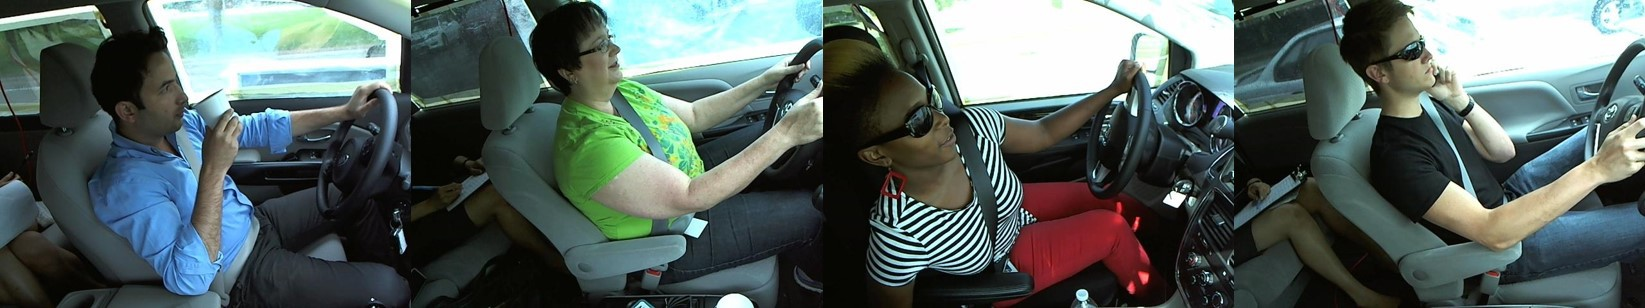
\includegraphics[width=\textwidth]{Chapters/Drive-Net/figures/image1.jpeg}
    \label{Drive-Net/figure1}
    \caption{Representative dashboard camera images of drivers being distracted. From left to right: drinking while driving; safe driving; reaching behind while driving; talking on the phone (left hand) while driving. \unskip~\protect\cite{1641075:26775858}}
\end{figure}


Object detection and human behavior detection are well-researched topics in the computer vision literature. \unskip~\cite{1641075:26775854} Machine learning (esp. Deep Learning) techniques can often learn complex models and achieve high accuracy, so many researchers have started to apply such techniques to solve computer vision problems, including object detection and human behavior detection. For example, the Inception-v4 model proposed by Szegedy \unskip~\cite{1641075:26775859} is a supervised learning model made up of deep convolutional residual networks (ResNet) that have more than 75 trainable layers, and achieves 96.92\% accuracy in the ImageNet data set. Girshick \unskip~\cite{1641075:26775856} introduced a very powerful method for object detection and segmentation using a region-based convolutional neural network (CNN). This method divides the human behavior detection problem into two problems. First, they apply an object detection algorithm to detect the regions of interest (ROIs) where people are present within an image. Next, each ROI is fed to a CNN to identify the type of behavior exhibited in the given ROI. Adding other traditional machine learning methods, such as ensemble learning (i.e. bagging) and K nearest neighbors (KNN), to the CNN model is a way to improve the accuracy of the already existing model. \unskip~\cite{1641075:26775847}

% \bgroup
\begin{figure*}[!htbp]
    \centering
    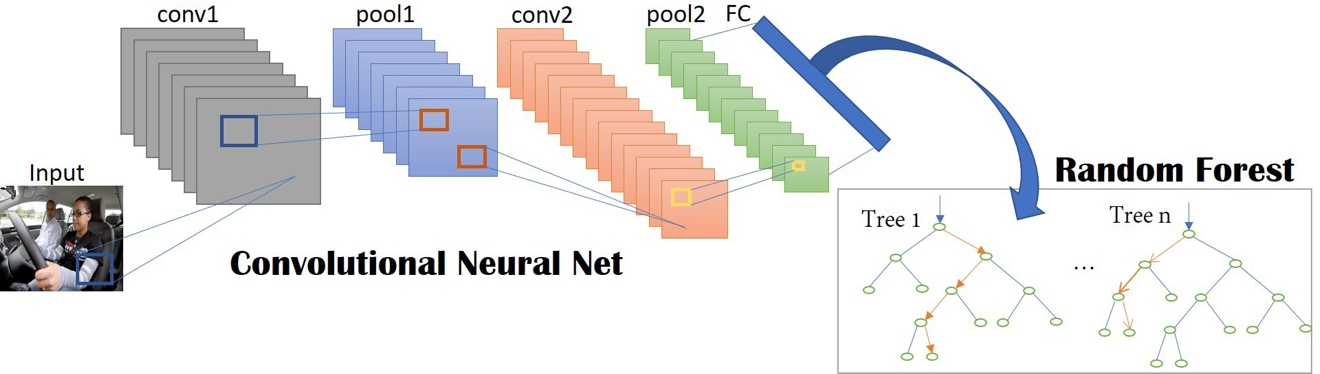
\includegraphics[width=\textwidth]{Chapters/Drive-Net/figures/image2.jpeg}
    \caption{An overview of the proposed Drive-Net. Our proposed CNN architecture (shown on the left side) consists of two convolution layers (conv), each followed by a maxpooling layer (pool), and a final ReLU layer, the output of which is regularized using dropouts to obtain a fully connected layer (FC). The FC layer is fed as input to the random forest classifier (on the right side), which predicts the final class label.}
    \label{Drive-Net/figure2}
\end{figure*}
% \egroup

One of the main drawbacks of CNN is that training the network using a large data set can lead to overfitting the model. To avoid this, ensemble methods such as random decision forests can be effective. With this in mind, we propose a new supervised learning algorithm called Drive-Net that combines a CNN and a random forest in a cascading fashion for application to the problem of driver distraction detection using dashboard camera images. We compare our proposed Drive-Net to two other neural network methods: a residual neural network (RNN) and a multilayer perceptron (MLP). We show that Drive-Net achieves better classification accuracy than the driver distraction detection algorithms that were proposed in the Kaggle competition. \unskip~\cite{1641075:26775858}

\section{Methods}
Our proposed method, Drive-Net, is a cascaded classifier consisting of two stages: a CNN as the first stage, whose output layer is fed as input to a random decision forest to predict the final class label. We define each stage in detail below.



\subsection{Convolutional Neural Network Configurations} We adopted the U-Net architecture \unskip~\cite{1641075:26775850} as the basis for our CNN. The motivation behind this architecture is that the contracting path captures the context around the objects to provide a better representation of the object compared to architectures such as AlexNet \unskip~\cite{1641075:26775852} and VGGNet \unskip~\cite{1641075:26775860} Very large networks like AlexNet and VGGNet require learning a massive number of parameters and are very difficult to train in general, needing significant computational time. Thus, we empirically modified the U-Net architecture in this work to suit our application.

To construct our CNN, we discard U-Net's layers of up-convolution and the last two layers of down-sampling and replace them with a $1\times1 $ convolution instead to obtain a fully connected layer. We use the rectifier activation function \unskip~\cite{1641075:26775860} for our CNN as the constant gradient of rectified linear units (ReLU) results in faster learning and reduces the problem of vanishing gradient compared to the hyperbolic tangent (${{tanh}{\left(\bullet\right)}} $). We implement a maximum-pooling layer instead of average-pooling in the subsampling layer. We observed that the performance is better when a ReLU layer was configured with the maximum pool layer, resulting in higher classification accuracy after 50 epochs. We use the $1\times1 $ convolutional filter for the Adam \unskip~\cite{1641075:26775857} optimizer. All other parameters, such as the number of layers, the size of the convolutional kernel, the training algorithm, and the number of neurons in the final dense layer, were experimentally determined for our application.

To keep the training time small, we reduced the size of the dashboard camera images by a factor of 10 by making them 64 \ensuremath{\times} 48 in size and feed them as input to our CNN. We do not zero-pad the image patches, as the ROI of human activity is located toward the center of the image. Two consecutive convolutional layers are used in the network. The first convolutional layer consists of 32 kernels of size $5\times5\times1 $. The second convolutional layer consists of 64 kernels of size $5\times5\times32 $. The subsampling layer is set as the maximum value in nonoverlapping windows of size $2\times2 $ (stride of 2). This reduces the size of the output of each convolutional layer by half. After the two convolutional and subsampling layers, we use a ReLU layer, where the activation y for a given input x is obtained as
\let\saveeqnno\theequation
\let\savefrac\frac
\def\dispfrac{\displaystyle\savefrac}
\begin{eqnarray}
\let\frac\dispfrac
\gdef\theequation{1}
\let\theHequation\theequation
\label{disp-formula-group-e98e45e883854b6aa2d919dcc0573fee}
\begin{array}{@{}l}y=f\left(x\right)=\text{max}(0,x)\end{array}
\end{eqnarray}
\global\let\theequation\saveeqnno
\addtocounter{equation}{-1}\ignorespaces
A graphical representation of the architecture of the proposed CNN model is shown in Figure~\ref{Drive-Net/figure2}  (see the left side).


\subsection{Random Decision Forest}A random forest classifier consists of a collection of decision tree classifiers combined to predict the class label, where each tree is grown in a randomized fashion. Each decision tree classifier consists of decision (or split) nodes and prediction (or leaf) nodes. The prediction nodes of each tree in the random forest classifier are labeled by the posterior distribution over the image classes. \unskip~\cite{1641075:26775861} Each decision node contains a test that best splits the space of the data to be classified. An image is classified by sending it down the decision tree and aggregating the posterior distributions that are reached. Most of the time, randomness is added to training at two points: when subsampling the training data and when choosing node tests. Each tree within the random forest classifier is binary and grows top-down. At each node, we select the binary test to maximize the information gain obtained by partitioning the training set $Q$ of image patches into two sets $Q_i$ according to the test.

\let\saveeqnno\theequation
\let\savefrac\frac
\def\dispfrac{\displaystyle\savefrac}
\begin{eqnarray}
\let\frac\dispfrac
\gdef\theequation{2}
\let\theHequation\theequation
\label{disp-formula-group-d27d73835da3454a817782924579e245}
\begin{array}{@{}l}\Delta E=-{\sum_i{\frac{\left(Q_i\right\vert}{\left(Q\right\vert}E\left(Q_i\right)}}\end{array}
\end{eqnarray}
\global\let\theequation\saveeqnno
\addtocounter{equation}{-1}\ignorespaces

Here $E\left(\cdot\right) $\ensuremath{_{}}is the entropy of the set and $\left\vert \cdot\right\vert $\ensuremath{_{}}is the size of the set. We repeat this selection process for each decision node until it reaches a certain depth. Many implementations of random forests \unskip~\cite{1641075:26775846}, \unskip~\cite{1641075:26775849} use simple pixel-level tests at the nodes because it results in faster tree convergence. As we are interested in features that encode shape and appearance, we are interested in spatial correspondence between pixels. Therefore, we use a simple test proposed by Bosch \unskip~\cite{1641075:26775861} {\textemdash} as a linear classifier on the characteristic vector {\textemdash} at each decision node.

Suppose that $T $ is the set of all trees, $C $ is the set of all classes, and $L $ is the set of all leaves for a given tree. During training, posterior probabilities $P_{t,l}\left(Y\left(I\right)=c\:\right) $ for each class $c\in C $ are found at each leaf node $l\in L $ for each tree $t\in T $. These probabilities are calculated as the ratio of the number of images $I $ of class $c $ that reach a leaf node $l $ to the total number of images that reach that leaf node $l $. $Y\left(I\right) $ is the class label of image $I $. During test time, we pass a new image through every decision tree until it reaches a prediction (or leaf) node, average all the posterior probabilities, and classify the image as

\let\saveeqnno\theequation
\let\savefrac\frac
\def\dispfrac{\displaystyle\savefrac}
\begin{eqnarray}
\let\frac\dispfrac
\gdef\theequation{3}
\let\theHequation\theequation
\label{disp-formula-group-032e1395024b44bca0feeb46474c0adc}
\begin{array}{@{}l}\widehat Y\left(I\right)=\underset c{\text{argmax}}\left\{\frac1{\left\vert T\right\vert}\sum_{t=1}^{\left\vert T\right\vert}P_{t,l}\left(Y\left(I\right)=c\right)\right\}\end{array}
\end{eqnarray}
\global\let\theequation\saveeqnno
\addtocounter{equation}{-1}\ignorespaces

where $l $ is the leaf node reached by the image $I $ in the tree $t $. A graphical representation of the proposed random forest classifier is shown in Figure~\ref{Drive-Net/figure2}  (see the right side).

\section{Experiments and Results}


\subsection{Data set} The Kaggle competition \unskip~\cite{1641075:26775858} for driver distraction has provided 22425 images for training and 79727 for tests. Since we did not have access to the test labels, our experiments were done solely on the training images. However, the quality and conditions of the training and testing images are similar; the only difference is that none of the drivers used in the training data set appear in the images in the test data set. The images are of size 640 \ensuremath{\times} 480, and for our experiments we converted them from color to grayscale.

Ten classes are provided, related to the ones listed in Section I. Each class includes almost tens of the data, so that we have a uniform distribution of sample data.

\begin{itemize}
  \item \relax c0: safe driving
  \item \relax c1: texting (right hand)
  \item \relax c2: talking on the phone (right hand)
  \item \relax c3: texting (left hand)
  \item \relax c4: talking on the phone (left hand)
  \item \relax c5: operating the radio
  \item \relax c6: drinking
  \item \relax c7: reaching behind
  \item \relax c8: hair and makeup
  \item \relax c9: talking to a passenger
\end{itemize}



\subsection{Algorithm Parameters}The convolutional neural random forest classifier is implemented using TensorFlow, \unskip~\cite{1641075:26775853} and runs on an NVIDIA GeForce GTX TITAN X GPU with 16 GB of memory. The classifier was trained using the Adam stochastic gradient descent algorithm \unskip~\cite{1641075:26775857} to efficiently optimize CNN weights. The weights were normalized using initialization as proposed in Kingma \unskip~\cite{1641075:26775857} and updated in a mini-batch scheme of 128 candidates. The biases were initialized with zero and the learning rate was set at $\alpha\;=\;0.001 $. The exponential decay rates for the estimates for the first and second moments were set as $\beta_1\;=\;0.9 $ and $\beta_2\;=\;0.99 $, respectively. We used $\epsilon={10}^{-8} $ to prevent division by zero. A dropout rate of $0.5 $ was implemented as regularization, applied to the output of the last convolutional layer and the dense layer to avoid overfitting. Finally, we used an epoch size of 50.  SoftMax loss (cross-entropy error loss) was used to measure the error loss. We used 100 estimators and a keep rate of $\gamma\;=\;{10}^{-4} $ for the random forest algorithm.


\subsection{Performance Evaluation} We tested the algorithm performance by performing k-fold cross-validation on the entire dataset. For our experiments, we varied the values of $k\in\lbrack2,\;5\rbrack $ and found that the results were consistent enough to indicate that the network is not overfitting. Therefore, we chose $k\;=\;5 $. First, we randomly choose the order of the driver images within the data set. For each fold of the k-fold cross-validation, we chose 80\% of the 22425 images as the training data set and tested the trained model on the remaining 20\% of the images. We ensured that the images from the entire dataset appeared in the test dataset only once in all k-folds, thereby allowing each image to be classified as a test image exactly once.

We compared our proposed Drive-Net with two other neural network classifiers: an RNN classifier, \unskip~\cite{1641075:26775863} and an MLP classifier \unskip~\cite{1641075:26775862}. We report the classification accuracy, which is defined as the percentage of correct predictions and the number of false positives (a.k.a. false detections) for each class, as the figures of merit for comparing the algorithms. For classification precision, we present the results of seven other methods based on support vector machines (SVMs), dimensionality reduction techniques such as principal component analysis (PCA), feature extraction techniques such as histogram of oriented gradients (HOG), very deep convolutional nets such as VGG-16, VGG-GAP, and an ensemble of these two as reported by Zhang \unskip~\cite{1641075:26775851} using the same Kaggle dataset of 22425 images.

Table~\ref{Drive-Net/Table1} shows the mean classification accuracy of the different classifiers as reported by Zhang \unskip~\cite{1641075:26775851} and that of the three neural network classifiers that we implemented. From Table~\ref{Drive-Net/Table1}, we observe that Drive-Net achieves a classification accuracy of 4.8\% points higher than the VGG-16 classifier, $3.7\% $ points higher than a VGG-GAP classifier, 2.4\% points higher than an ensemble of VGG-16 and VGG-GAP classifiers, 3.3\% points higher than the RNN classifier and 13\% points higher than the MLP classifier.


\begin{table}[!htbp]
\caption{Mean Classification Accuracy of Automated Methods}
\label{Drive-Net/Table1}
\def\arraystretch{1}
\ignorespaces
\centering
\begin{tabulary}{\linewidth}{p{\dimexpr.61620000000000005\linewidth-2\tabcolsep}p{\dimexpr.38379999999999995\linewidth-2\tabcolsep}}
\hline Method & Accuracy\\
\hline
\multicolumn{2}{>{\centering\arraybackslash}p{\dimexpr(1\linewidth-2\tabcolsep)}}{\cellcolor[HTML]{CCCCCC}\textit{Methods from Zhang \unskip~\cite{1641075:26775851}}}\\
 Pixel SVC &
   18.3\%\\
 SVC + HOG &
   28.2\%\\
 SVC + PCA &
   34.8\%\\
 SVC + BBox + PCA &
   40.7\%\\
 VGG-16 &
   90.2\%\\
 VGG-GAP &
   91.3\%\\
 Ensemble VGG-16 and VGG-GAP &
   92.6\%\\\cline{1-1}
\multicolumn{2}{>{\centering\arraybackslash}p{\dimexpr(1\linewidth-2\tabcolsep)}}{\cellcolor[HTML]{CCCCCC}\textit{Methods we implemented:}}\\
 MLP &
   82\%\\
 RNN &
   91.7\%\\
 Drive-Net &
   95\%\\
\hline
\end{tabulary}\par
\end{table}


Table~\ref{Drive-Net/Table2} shows the number of false classifications for our Drive-Net and for RNN and MLP. From Table~\ref{Drive-Net/Table2}, we observe that our Drive-Net can identify the classes c6 (drinking) and c3 (texting with left hand) with minimum false detections, while the RNN and MLP classifiers have a hard time distinguishing these classes with many false detections, usually higher than the number of false detections in the other classes of these methods. Also, the total number of false detections for our Drive-Net is an order of magnitude smaller than that of the MLP classifier and slightly smaller compared to the RNN classifier.

\begin{table}[!htbp]
\caption{Class's Error Count for Neural Network Methods}
\label{Drive-Net/Table2}
\def\arraystretch{1}
\ignorespaces
\centering
\begin{tabulary}{\linewidth}{LLLL}
\hline Class &  Drive-Net & MLP & RNN\\
\hline
 c0 &
   35 &
   356 &
   48\\
 c1 &
   17 &
   199 &
   34\\
 c2 &
   14 &
   158 &
   31\\
 c3 &
   09 &
   116 &
   47\\
 c4 &
   34 &
   252 &
   30\\
 c5 &
   15 &
   108 &
   14\\
 c6 &
   08 &
   263 &
   18\\
 c7 &
   21 &
   117 &
   10\\
 c8 &
   29 &
   181 &
   46\\
 c9 &
   26 &
   268 &
   46\\

\cellcolor[HTML]{CCCCCC}{ All Classes} &
  \cellcolor[HTML]{CCCCCC}{ 208} &
  \cellcolor[HTML]{CCCCCC}{ 2018} &
  \cellcolor[HTML]{CCCCCC}{ 324}\\
\hline
\end{tabulary}\par
\end{table}


\section{Conclusion}
Distracted driving is one of the main causes of motor vehicle accidents. Therefore, there is a significant interest in finding automated methods to recognize signs of driver distraction from dashboard camera images installed in vehicles. We propose a solution to this problem using a supervised learning framework. Our method, named Drive-Net, combines a CNN and a random forest classifier to recognize the various categories of driver distraction in images. We apply our Drive-Net to a publicly available dataset of images used in a Kaggle competition and show that our Drive-Net achieves better accuracy than the driver-distraction algorithms reported in the competition. We also compared Drive-Net to two other neural network algorithms: an RNN and an MLP algorithm, using the same data set. The results show that DriveNet achieves better detection accuracy compared to the other two algorithms.

% trigger a \newpage just before the given reference
% number - used to balance the columns on the last page
% adjust value as needed - may need to be readjusted if
% the document is modified later
%\IEEEtriggeratref{8}
% The "triggered" command can be changed if desired:
%\IEEEtriggercmd{\enlargethispage{-5in}}


% references section
\bibliographystyle{ieeetr}
\bibliography{Chapters/Drive-Net/Drive-Net}

\subfile{Chapters/Drive-Net/Drive-Net.tex}
% \subfile{Chapters/crowd/main.tex}
\subfile{Chapters/Thalamus/thalamus}
% \include{Chapters/crowd/crowd_for_thesis}

\printindex
% %% ================================================================
\begin{thebibliography}{}

\bibitem[DF]{bib:df}
D.S.~Dummit and R.M.~Foote.
\newblock {\em Abstract Algebra} (2nd ed.).
\newblock John Wiley and Sons, 1999.

\bibitem[Golomb]{bib:golomb}
Golomb,~S.W.
\newblock {\em Random permutations}.
\newblock Bull. Amer. Math. Soc. 70 (1964), 747.

\bibitem[HN]{bib:HN}
Hunter,~J. and Nachtergaele,~B.
\newblock {\em Applied Analysis}.
\newblock World Scientific, 2001.

\bibitem[FG]{bib:fg}
Fristedt,~B. and Gray,~L.
\newblock {\em A Modern Approach to Probability Theory}.
\newblock Birkh\"auser, 1997.

\bibitem[Lugo]{bib:lugo}
Lugo,~M.
\newblock {\em Profiles of permutations.}
\newblock Electronic Journal of Combinatorics, \textbf{16} (2009) R99.

\bibitem[NR]{bib:nr}
Press,~W. et al.
\newblock {\em Numerical Recipes} (2nd ed.).
\newblock Cambridge, 1992.

\end{thebibliography}


%% ================================================================
\end{document}
